\documentclass{article}
\usepackage{preamble}
\usepackage{preamble_style}

\def\Ra{\mathrm{Ra}}
\def\Pr{\mathrm{Pr}}
\def\Le{\mathrm{Le}}

\title{Thermohaline circulation}
\author{Víctor Ballester and Victor Botez}
\date{\parbox{\linewidth}{\centering
Computational Fluid Dynamics\endgraf
M2 - Applied and Theoretical Mathematics\endgraf
Université Paris-Dauphine, PSL\endgraf
\today}}

\begin{document}

\maketitle

\section{Introduction}
The thermohaline circulation is a global circulation of the ocean that is driven by the density differences due to temperature and salinity. It is a key component of the Earth's climate system and plays a crucial role in the heat transport from the equator to the poles. The circulation is driven by the sinking of cold and salty water in the North Atlantic and the upwelling of warm and less salty water in the Southern Ocean. The thermohaline circulation is a complex and nonlinear system that is influenced by a variety of factors, including temperature, salinity, wind, and ocean currents. In this project, we aim to study the thermohaline circulation using a simplified mathematical model based on the Navier-Stokes equations and the advection-diffusion equations for temperature and salinity. We will investigate the stability and bifurcation of the circulation patterns as a function of the Rayleigh number, the Prandtl number, and the Lewis number.

\section{Theoretical model}
\subsection{Governing equations}
To model the thermohaline convection we implement the Navier-Stokes equations with a gravity forcing and the advection-diffusion equations for temperature and salinity. The equations are given by:
\begin{equation}
  \begin{aligned}
    \rho\left(\frac{\partial\mathbf{u}}{\partial t} + (\mathbf{u}\cdot\nabla)\mathbf{u}\right) & = -\nabla P + \rho\nu\nabla^2\mathbf{u} + \rho \mathbf{g} \\
    \pdv{\rho}{t} + \nabla\cdot(\rho\mathbf{u})                                                & = 0                                                       \\
    \frac{\partial T}{\partial t} + (\mathbf{u}\cdot\nabla)T                                   & = \kappa_T \nabla^2T                                      \\
    \frac{\partial S}{\partial t} + (\mathbf{u}\cdot\nabla)S                                   & = \kappa_S \nabla^2S                                      \\
  \end{aligned}
\end{equation}
These equations can be simplified by introducing the Boussinesq approximation, which assumes that the density variations are small. Moreover, after performing a Taylor expansion of the density of the water around some equilibrium value $\rho_0$ yet to be defined, and assuming that it depends only on the temperature and the salinity we get:
\begin{equation}
  \rho = \rho_0(1-\alpha_T\Delta T + \alpha_S\Delta S)
\end{equation}
with $\alpha_T:= -\frac{1}{\rho_0}\frac{\partial\rho}{\partial T}$ and $\alpha_S:= \frac{1}{\rho_0}\frac{\partial\rho}{\partial S}$ are the thermal and saline expansion coefficients respectively. From here on, the notation $\Delta A$ will always denote a variation of the quantity $A$, while the laplacian of $A$ will be expressed as $\nabla^2A$. It is a known fact that these two values, $\alpha_T$ and $\alpha_S$ are positive for water. This implies that whenever the temperature increases, the water density decreases and contrarily whenever the salinity increases, so does the water density. So if we interpret the $\rho\mathbf{g}$ term as a forcing term (which is not really the case since the velocity is involved into their evolution equations through the transport term) we already see that the effect related to the two will be opposite.

Now introducing the $\rho_0\mathbf{g}=-\rho_0g\vf{e}_z$ into the pressure gradient and writing all equations at zero order in density except the buoyancy part (Boussinesq approximation), one gets:
\begin{equation}\label{eq:boussinesq}
  \begin{aligned}
    \frac{\partial\mathbf{u}}{\partial t} + (\mathbf{u}\cdot\nabla)\mathbf{u} & = -\nabla p+ \nu\nabla^2\mathbf{u} + (\alpha_T\Delta T - \alpha_S\Delta S)g\vf{e}_z \\
    \frac{\partial T}{\partial t} + (\mathbf{u}\cdot\nabla)T                  & = \kappa_T \nabla^2T                                                                \\
    \frac{\partial S}{\partial t} + (\mathbf{u}\cdot\nabla)S                  & = \kappa_S \nabla^2S                                                                \\
    \nabla\cdot\mathbf{u}                                                     & = 0
  \end{aligned}
\end{equation}
for some appropriate $p$.

\subsection{Boundary conditions}\label{sec:boundary_conditions}
We will consider a two-dimensional rectangular domain $(x,z) \in [0,L]\times[0,h]$ with the top boundary representing the interface between the ocean and the atmosphere and the bottom boundary representing the ocean floor. We will impose the following boundary conditions:
\begin{itemize}
  \item On the two sides $x = 0$ and $x = L$ we consider Neumann boundary conditions for every quantity.
  \item At the bottom of the ocean $z = 0$ we impose a constant temperature and salinity and no slip condition for the velocity field.
  \item At the surface $z = h$ we impose free slip condition for the velocity field and a flux of temperature and salinity.
\end{itemize}

Our aim was to understand the convection in the ocean from one pole to the other, passing through the equator. Thus, $x=0$ and $x=L$ represent the poles and $x=L/2$ represents the equator.
In order to correctly define the fluxes of temperature and salinity, we want to impose that the ocean loses heat at the poles and absorbs heat at the equator and that the salinity decreases (because of the melting of ice) at the poles and increases at the equator (because of the evaporation of water). In the end, taking into account all these boundary conditions we consider the following Neumann conditions:
\begin{equation}
  \begin{aligned}
    \frac{\partial T}{\partial z}\bigg|_{z = h} & = -T_0\cos(2\pi \frac{x}{L}) \\
    \frac{\partial S}{\partial z}\bigg|_{z = h} & = -S_0\cos(2\pi \frac{x}{L})
  \end{aligned}
\end{equation}


\subsection{Dimensionless equations}
In order to simplify the equations and make them easier to work with, we introduce dimensionless variables. Introducing a characteristic length $h$ (the depth of the ocean), a characteristic velocity $U$, which we impose it to be such that the advection term is of the same order as the viscous term for the temperature, we get a value $U=\frac{\kappa_T}{h}$. This leads to a characteristic time $\tau = \frac{h^2}{\kappa_T}$.

We stress out from now that the Taylor expansion in the Boussinesq approximation in \cref{eq:boussinesq} are performed near an equilibrium value $\rho_0$. So an issue to be addressed is how to define the temperature and salinity at this equilibrium value. A first attempt to define these quantities was given using the profile obtained when solving $\nabla^2T = 0$ and $\nabla^2S=0$ with the appropriate boundary conditions, which we called the conduction temperature (the stationary profile that is obtained when removing the advection term). But the results were completely opposite to what we were expecting, and we therefore decided to drop this idea to finally just take as equilibrium value the one at the bottom.

Following in the same line of thought, we introduce the following dimensionless variables for the temperature and salinity as $\tilde{T} = \frac{\Delta T}{T_0}$ and $\tilde{S} = \frac{\Delta S}{S_0}$. Thus, after dropping the tildes, the dimensionless equations become:

\begin{equation}
  \begin{aligned}
    \frac{\partial\mathbf{u}}{\partial t} + (\mathbf{u}\cdot\nabla)\mathbf{u} & = -\nabla p + \frac{\nu}{\kappa_T}\nabla^2\mathbf{u} + g h^3\left(\frac{\alpha_T T_0}{\kappa_T^2} T - \frac{\alpha_S S_0}{\kappa_T^2} S\right)\vf{e}_z \\
    \frac{\partial T}{\partial t} + (\mathbf{u}\cdot\nabla)T                  & = \nabla^2T                                                                                                                                            \\
    \frac{\partial S}{\partial t} + (\mathbf{u}\cdot\nabla)S                  & = \frac{\kappa_S}{\kappa_T}\nabla^2S                                                                                                                   \\
    \nabla\cdot\mathbf{u}                                                     & = 0
  \end{aligned}
\end{equation}

Introducing the Prandtl number $\Pr = \frac{\nu}{\kappa_T}$, the Rayleigh number $\Ra = \frac{\alpha_T g h^3 T_0}{\nu \kappa_T}$, the Lewis number $\Le = \frac{\kappa_T}{\kappa_S}$ and $R_{\rho} = \frac{\alpha_T T_0}{\alpha_S S_0}$, the final equations can be rewritten as:
\begin{equation}\label{eq:ns}
  \begin{aligned}
    \frac{\partial\mathbf{u}}{\partial t} + (\mathbf{u}\cdot\nabla)\mathbf{u} & = -\nabla p + \Pr\nabla^2\mathbf{u} + \Pr\Ra\left(T - \frac{1}{R_{\rho}}S\right)\vf{e}_z \\
    \frac{\partial T}{\partial t} + (\mathbf{u}\cdot\nabla)T                  & = \nabla^2T                                                                              \\
    \frac{\partial S}{\partial t} + (\mathbf{u}\cdot\nabla)S                  & = \frac{1}{\Le}\nabla^2S                                                                 \\
    \nabla\cdot\mathbf{u}                                                     & = 0
  \end{aligned}
\end{equation}

The first thing to notice is that both the temperature and the salinity are important in these equations up to a constant so that we can choose to have the boundary conditions $T|_{z=0} = 0$ and $S|_{z=0} = 0$.

The Prandtl number $\Pr$ is the viscosity of the Navier-Stokes equation, which we choose to keep constant in our simulations. The Rayleigh number $\Ra$ can be seen as the amplitude of the forcing term in the Navier-Stokes equation. It is a measure of the strength of the buoyancy force relative to the viscous force. The dimensionless parameter $R_\rho$ attempts to quantify the relative importance of temperature and salinity in the density of the fluid. Finally, the Lewis number $\Le$ concerns about the ratio between the thermal and saline diffusivities.

The initial conditions for our problem are taken to be zero velocity and pressure fields and a temperature and salinity field that solve the Poisson equation $\nabla^2T = 0$ and $\nabla^2S = 0$ with the boundary conditions that match the ones imposed above for these quantities. This aims to have a stable initial state (quasi stationary for those two fields) which will make the Boussinesq approximation valid. In our case, we took as solutions of these two equations:
\begin{equation}
  \begin{aligned}
    T_\mathrm{initial}(x,z) & = -A_T \cos\left(\frac{2\pi x}{L}\right) \sinh\left(\frac{2\pi z}{L}\right) \\
    S_\mathrm{initial}(x,z) & = -A_S \cos\left(\frac{2\pi x}{L}\right) \sinh\left(\frac{2\pi z}{L}\right)
  \end{aligned}
\end{equation}
where $A_T$ and $A_S$ are some normalization constants that match the boundary conditions on the top layer of the domain.

\section{Numerical method}

In this section we discuss our numerical solver to integrate \cref{eq:ns} together with the boundary conditions presented in \cref{sec:boundary_conditions}. To simplify the equations, we use \textit{Chorin's projection method}. The idea of the method is to first predict the velocities for the next time step by solving the advection and the diffusion term. With the intermediate velocity field we solve the Poisson equation with a finite difference method (described below). Finally, the \textit{projection step} is preformed, and the velocity field is updated with the new pressure field.

This method is based on the Helmholtz-Hodge decomposition of a vector field $\vf{F}$, which states that any vector field can be decomposed into a sum of a solenoidal (divergence-free) and an irrotational (curl-free) part. In our case, this means that the velocity field $\vf{u}^*$ can be decomposed into a sum of a solenoidal part $\vf{u}^{n+1}$ and an irrotational part $\nabla p^{n+1}$, where $p^{n+1}$ is the pressure field at time $t^{n+1}$. The projection step is then used to enforce the incompressibility of the velocity field, and to update the velocity field with the new pressure field.

To ensure that the boundary conditions are met, we impose the conditions for the velocity right before solving the Poisson equation and at the end of each iteration. The boundary conditions for the pressure are imposed after solving the Poisson equation and before correcting the velocities in the projection step.

After completing the Chorin's projection method, with the new velocity field, we can update the temperature and salinity fields using a semi-Lagrangian method for the advection term and a central differences scheme for the diffusion term.

Next, we provide a summary of the steps in our method. Assuming we know the velocity field at time $t^n$, $\vf{u}^n$, we want to compute the velocity field at time $t^{n+1}$, $\vf{u}^{n+1}$.
\begin{enumerate}
  \item Solve for $\vf{u}^a$ in $\displaystyle  \frac{\vf{u}^a-\vf{u}^n}{\Delta t} + \vf{u}^n \cdot \nabla \vf{u}^n = 0$ using a semi-Lagrangian method.
  \item Solve for $\vf{u}^*$ in $\displaystyle  \frac{\vf{u}^* - \vf{u}^a}{\Delta t} = \Pr \nabla^2 \vf{u}^n +\Pr\Ra\left(T^n - \frac{1}{R_{\rho}}S^n\right)\vf{e}_z$ using a central differences scheme.
  \item Set the boundary conditions for the intermediate velocity field $\vf{u}^*$.
  \item Solve the Poisson equation for the pressure, $\displaystyle \nabla^2 p^{n+1} = \frac{1}{\Delta t}\nabla \cdot \vf{u}^*$.
  \item Set the boundary conditions for the pressure $p^{n+1}$.
  \item Project the pressure to the intermediate velocity to obtain the new velocity at time $t^{n+1}$, $\displaystyle \vf{u}^{n+1} = \vf{u}^* - \Delta t\nabla p^{n+1}$.
  \item Set the boundary conditions for the velocity field $\vf{u}^{n+1}$.
  \item Solve for $T^{a}$ in $\displaystyle  \frac{T^{a}-T^{n}}{\Delta t} + \vf{u}^{n+1} \cdot \nabla T^{n} = 0$ and for $S^{a}$ in $\displaystyle  \frac{S^{a}-S^{n}}{\Delta t} + \vf{u}^{n+1} \cdot \nabla S^{n} = 0$ using a semi-Lagrangian method.
  \item Solve for $T^{n+1}$ in $\displaystyle  \frac{T^{n+1}-T^{a}}{\Delta t} = \nabla^2 T^{n}$ and for $S^{n+1}$ in $\displaystyle  \frac{S^{n+1}-S^{a}}{\Delta t} = \frac{1}{\Le}\nabla^2 S^{n}$ using a central differences scheme.
  \item Set the boundary conditions for the temperature and salinity fields $T^{n+1}$ and $S^{n+1}$.
\end{enumerate}
From these equations, one can easily check that we have:
\begin{align*}
  \frac{\vf{u}^{n+1}-\vf{u}^n}{\Delta t} + \vf{u}^n \cdot \nabla \vf{u}^n - \Pr \nabla^2 \vf{u}^n + \nabla p^{n+1} & = 0 \\
  \nabla \cdot \vf{u}^{n+1}                                                                                        & = 0 \\
  \frac{T^{n+1}-T^{n}}{\Delta t} + \vf{u}^{n+1} \cdot \nabla T^{n} - \nabla^2 T^{n}                                & = 0 \\
  \frac{S^{n+1}-S^{n}}{\Delta t} + \vf{u}^{n+1} \cdot \nabla S^{n} - \frac{1}{\Le}\nabla^2 S^{n}                   & = 0
\end{align*}

Recall that when solving the heat equations in steps 2 and 9 we must impose the stability condition $\kappa \Delta t\left( \frac{1}{{\Delta x}^2} + \frac{1}{{\Delta y}^2}\right) \leq \frac{1}{2}$, where $\kappa$ is the diffusive coefficient in each case. For us, $\kappa \in \{\Pr, 1, 1/\Le\}$ and thus can be quite high as $\Pr\sim 10$ for salt water. This means, assuming an homogeneous grid, that the time step must be less than or equal to $2.5\times 10^{-6}$ for a $\Delta x = \Delta y = 0.01$.

A first attempt to solve this high computational cost is to use an implicit method to solve the heat equation. That is, to transform steps 2.\ and 9.\ into:
\begin{enumerate}
  \setcounter{enumi}{1}
  \item Solve for $\vf{u}^*$ in $\displaystyle  \frac{\vf{u}^* - \vf{u}^a}{\Delta t} = \Pr \nabla^2 \vf{u}^* +\Pr\Ra\left(T^n - \frac{1}{R_{\rho}}S^n\right)\vf{e}_z$ using a central differences scheme.
        \setcounter{enumi}{8}
  \item Solve for $T^{n+1}$ in $\displaystyle  \frac{T^{n+1}-T^{a}}{\Delta t} = \nabla^2 T^{n+1}$ and for $S^{n+1}$ in $\displaystyle  \frac{S^{n+1}-S^{a}}{\Delta t} = \frac{1}{\Le}\nabla^2 S^{n+1}$ using a central differences scheme.
\end{enumerate}

This has the advantage to be unconditionally stable, leaving us only with the stability condition for the advection term. However, if we sum all the equations, we observe that we are actually solving:
\begin{align*}
  \frac{\vf{u}^{n+1}-\vf{u}^n}{\Delta t} + \vf{u}^n \cdot \nabla \vf{u}^n - \Pr \nabla^2 \vf{u}^{n+1} + \nabla p^{n+1} & = \Delta t \Pr \nabla^2(\nabla p^{n+1}) \\
  \nabla \cdot \vf{u}^{n+1}                                                                                            & = 0                                     \\
  \frac{T^{n+1}-T^{n}}{\Delta t} + \vf{u}^{n+1} \cdot \nabla T^{n} - \nabla^2 T^{n+1}                                  & = 0                                     \\
  \frac{S^{n+1}-S^{n}}{\Delta t} + \vf{u}^{n+1} \cdot \nabla S^{n} - \frac{1}{\Le}\nabla^2 S^{n+1}                     & = 0
\end{align*}

We observe that method is consistent with the original problem only if the derivatives of the pressure are bounded. With our explicit solver we checked that that was actually our case and so it makes sense to use the implicit method to solve the heat equations.

% \begin{figure}[ht]
%   \centering
%   \begin{subfigure}{0.45\textwidth}
%     \centering
%     \includegraphics[width=\textwidth]{images/pressure_data/la
%     \caption{Pressure and pressure gradients at time $t=0.1$}
%   \end{subfigure}
%   \begin{subfigure}{0.45\textwidth}
%     \centering
%     \includegraphics[width=\textwidth]{figures/implicit_stability.png}
%     \caption{Laplacian of the gradients of the pressure at time $t=0.1$}
%   \end{subfigure}
%   \caption{Pressure and pressure derivatives at time $t=0.1$ to check the consistency of the implicit method.}
%   \label{fig:pressure}
% \end{figure}

With this approach we can now increase the time step to $\Delta t = 10^{-3}$ and still have a stable method. This is a huge improvement in terms of computational cost as we can extend the simulation time.

\section{Results}
We carried out two different simulations, one with the explicit method and another with the implicit method. The parameters used in the simulations are $\Pr = 10$, $\Ra = 10$. The other parameters, $\Le$ and $R_{\rho}$, are left free.

\subsection{Convection phase diagram}
In this section we aim to study in which cases we have a temperature convection or a salinity convection of the flow. The first one is characterized by the flow moving upwards in the center of the domain (equator) and downwards at the extremities (poles). The second one is characterized by the flow moving upwards at the poles and downwards at the equator. We will study the phase diagram of the convection patterns as a function of the Lewis number and the $R_{\rho}$ parameter.

Since $R_\rho=1$ is the critical value for which the temperature and salinity have the same importance in the density of the fluid, we will focus our in a slight variation of this value. We will consider $R_\rho \in [0.9,1.1]$ and $\Le\in \{0.01, 0.1, 1, 10, 100\}$. \cref{fig:phase_diagram} shows the phase diagram of the convection patterns.

\begin{figure}[ht]
  \centering
  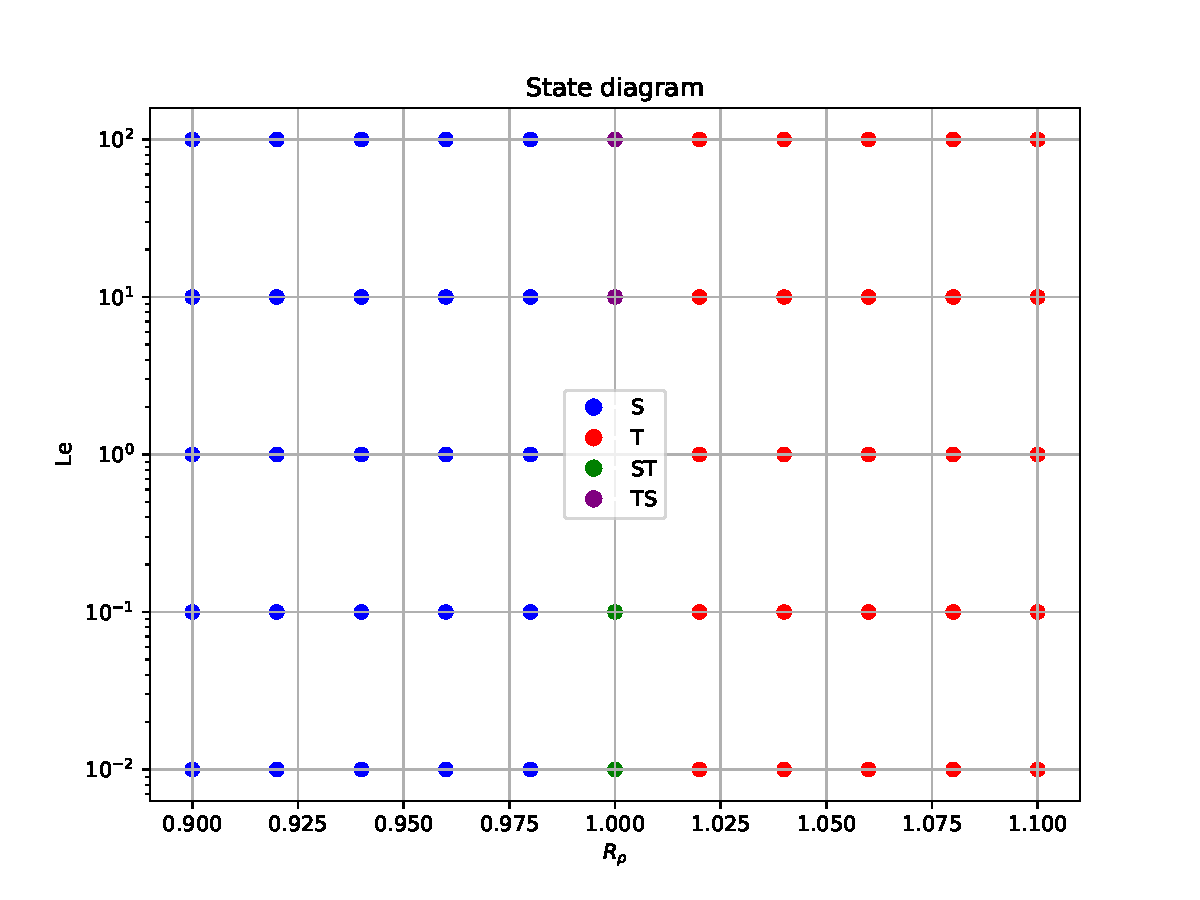
\includegraphics[width=0.6\textwidth]{images/phase_diagram.pdf}
  \caption{Phase diagram of the convection patterns as a function of the Lewis number and the $R_{\rho}$ parameter. The red dots represent the cases where we have temperature convection; the blue dots represent the cases where we have salinity convection; the green dots represent the cases where initially we have salinity convection but it transitions to temperature convection, and the purple dots represent the cases where initially we have temperature convection but it transitions to salinity convection.}
  \label{fig:phase_diagram}
\end{figure}

A first note to clarify is that we did not simulate the cases where $R_\rho=1$ and $\Le=1$, as it does not give any convection since the fields $T$ and $S$ are in that case the same and we start with null velocity fields in the domain.

As we can see in \cref{fig:phase_diagram}, we have a strong preference for salinity convection whenever $R_\rho<1$ and a strong preference for temperature convection whenever $R_\rho>1$. At $R_\rho=1$ we have a transition between the two and depending on the Lewis number we transition from one to the other or viceversa.

\begin{figure}[ht]
  \centering
  \begin{subfigure}{\textwidth}
    \centering
    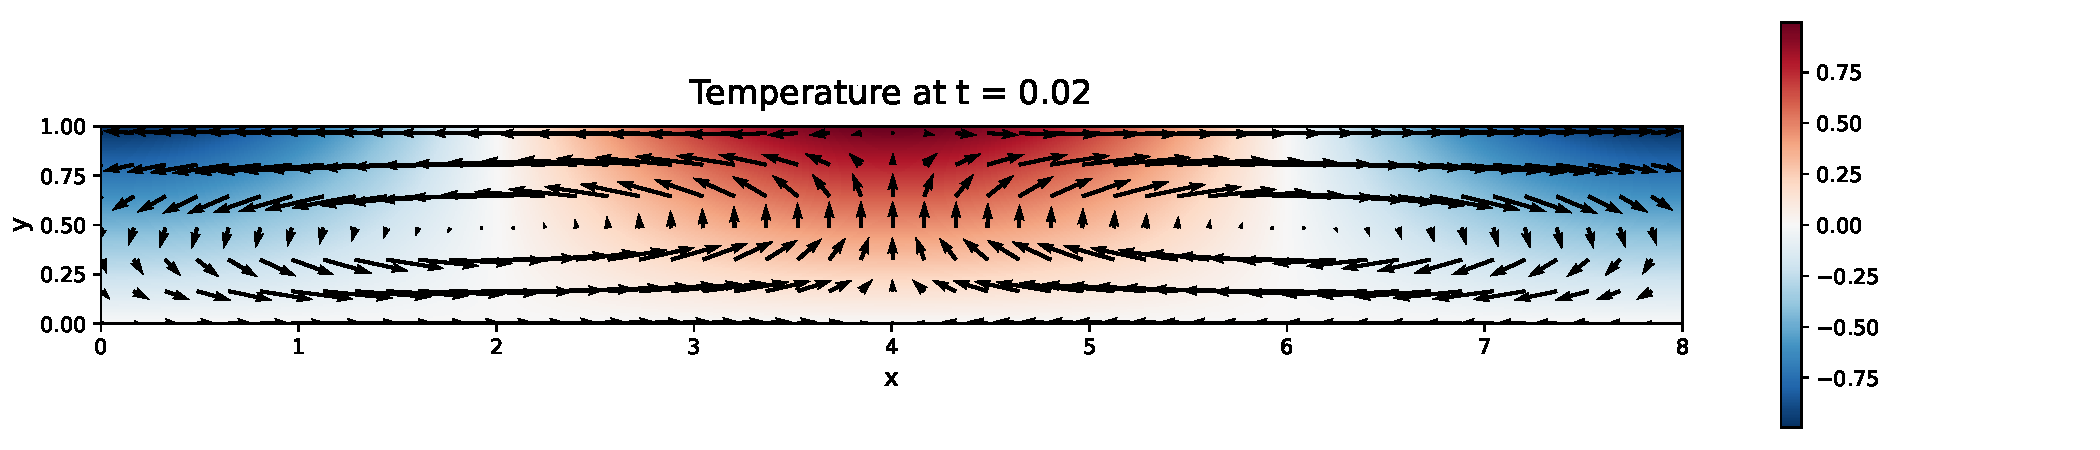
\includegraphics[width=\textwidth]{images/TS_1.pdf}
  \end{subfigure}\\
  \begin{subfigure}{\textwidth}
    \centering
    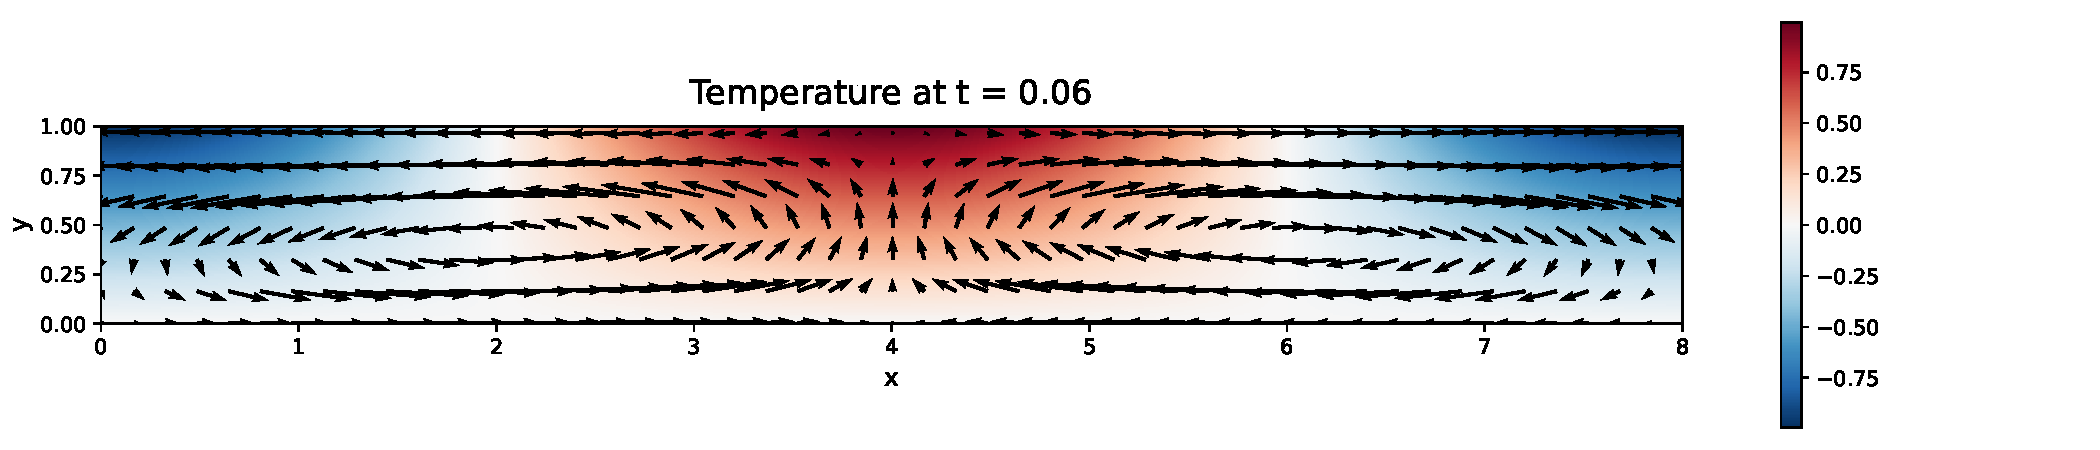
\includegraphics[width=\textwidth]{images/TS_2.pdf}
  \end{subfigure}\\
  \begin{subfigure}{\textwidth}
    \centering
    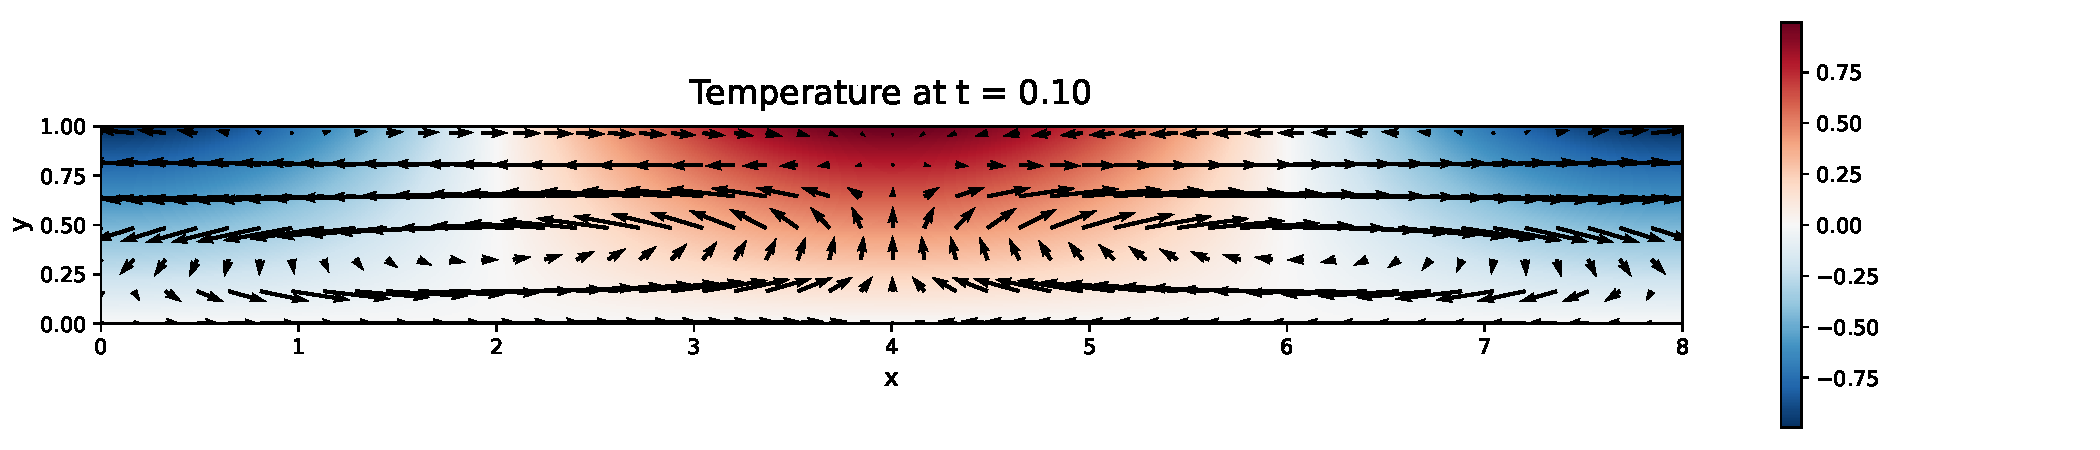
\includegraphics[width=\textwidth]{images/TS_3.pdf}
  \end{subfigure}\\
  \begin{subfigure}{\textwidth}
    \centering
    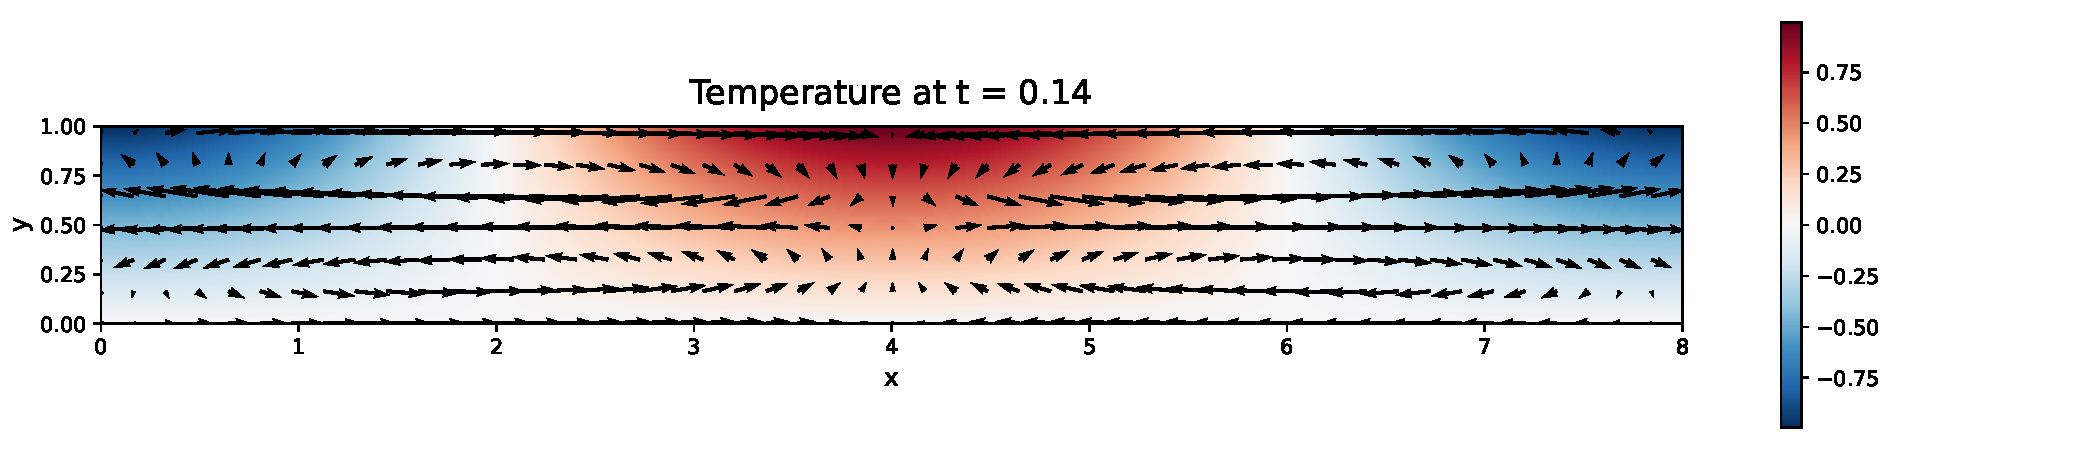
\includegraphics[width=\textwidth]{images/TS_4.pdf}
  \end{subfigure}\\
  \begin{subfigure}{\textwidth}
    \centering
    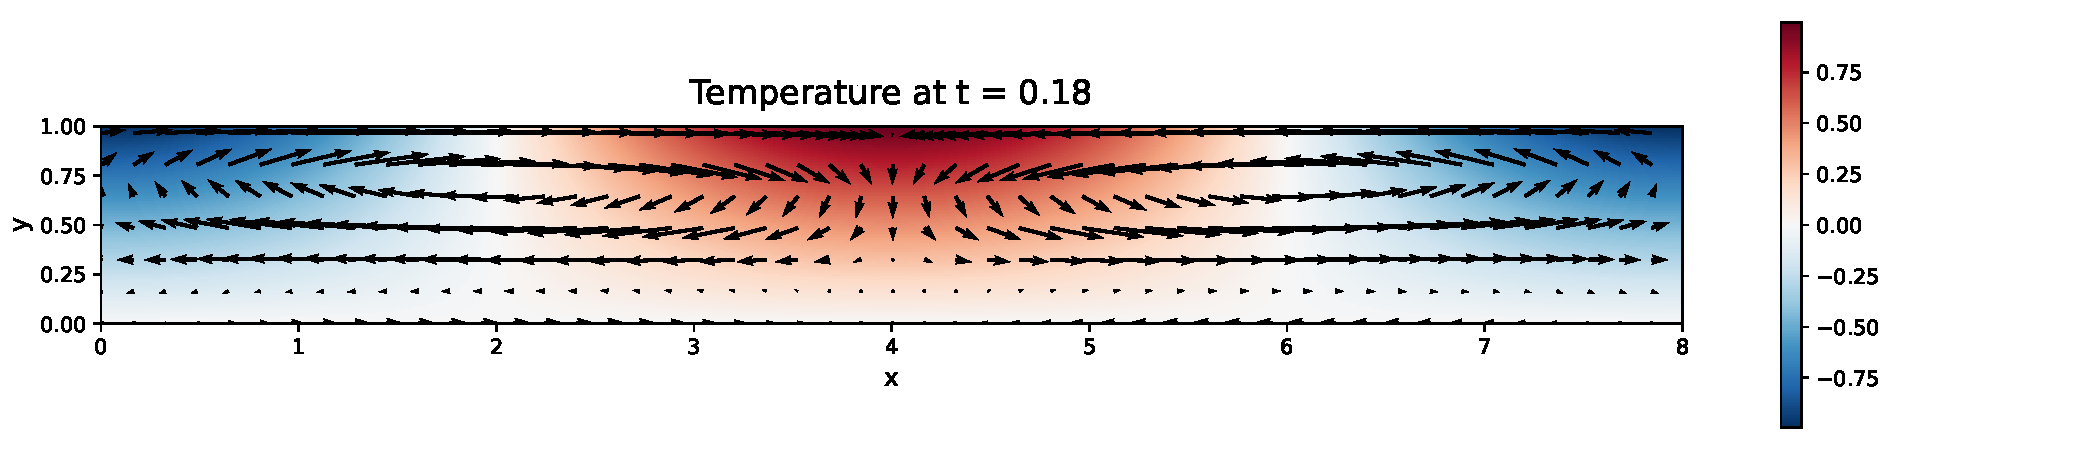
\includegraphics[width=\textwidth]{images/TS_5.pdf}
  \end{subfigure}\\
  \begin{subfigure}{\textwidth}
    \centering
    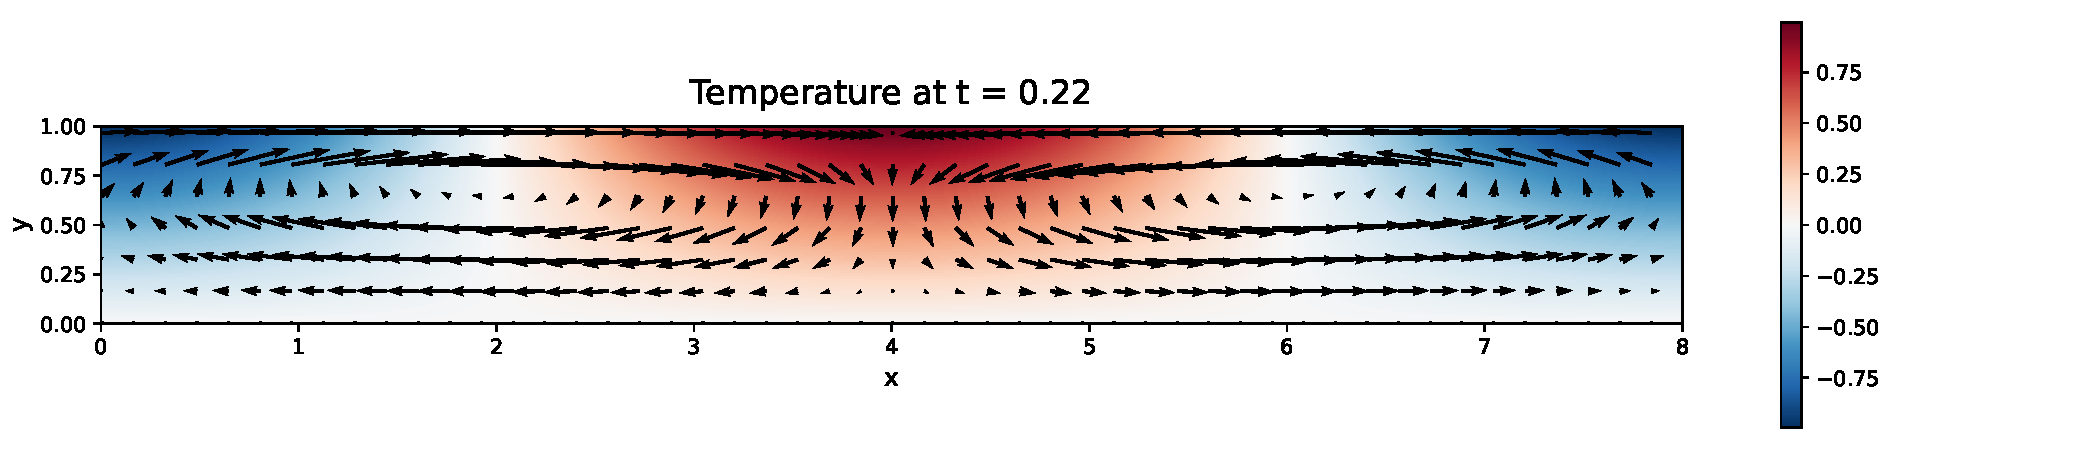
\includegraphics[width=\textwidth]{images/TS_6.pdf}
  \end{subfigure}\\
  \caption{Transition from a temperature convection to a salinity convection. The parameters used in this simulation are $\Pr = 10$, $\Ra = 10$, $\Le = 100$ and $R_{\rho} = 1$ and the spacing in the spatial grid is $\Delta x = \Delta y = 0.01$ and the time step is $\Delta t = 10^{-3}$.}
  \label{fig:changeTS}
\end{figure}

In \cref{fig:changeTS}, we can see the transition from a temperature convection to a salinity convection. The parameters used in this simulation are $\Pr = 10$, $\Ra = 10$, $\Le = 100$ and $R_{\rho} = 1$, together with $\Delta x = \Delta y = 0.01$ and $\Delta t = 10^{-3}$.

\subsection{french victor}

\section{Conclusions}
\end{document}
